\chapter{Систення інформація за допомогою бінарних дерев}
\nopagebreak[4]
\section*{Мета роботи}

\nopagebreak[4]
\section{Вступ}
\nopagebreak[4]
Дерево~--- це структура даних, що представляє собою сукупність елементів і відносин, що утворюють ієрархічну структуру цих елементів (рис.~\ref{f:tree1}). Кожен елемент дерева називається вершиною (вузлом) дерева. Вершини дерева з'єднані спрямованими дугами, які називають гілками дерева. Початковий вузол дерева називають коренем дерева, йому відповідає нульовий рівень. Листям дерева називають вершини, в які входить одна гілка і не виходить жодної гілки.

Кожне дерево має такі властивості:
\begin{itemize}
\item існує вузол, в який не входить ні однієї дуги (корінь);
    в кожну вершину, крім кореня, входить одна дуга.
\end{itemize}


Дерева особливо часто використовують на практиці при зображенні різних ієрархій.

\begin{figure}
\caption{Дерево}\label{f:tree1}
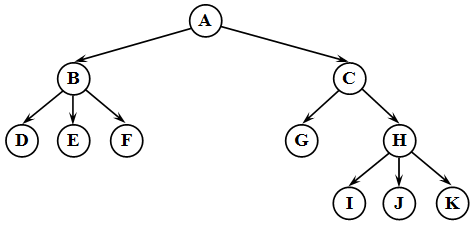
\includegraphics[width=13cm]{pic/31_01.png}

\end{figure}


Всі вершини, в які входять гілки, що виходять з однієї загальної вершини, називаються нащадками, а сама вершина - предком. Для кожного предка може бути виділено кілька. Рівень нащадка на одиницю перевищує рівень його предка. Корінь дерева не має предка, а листя дерева не мають нащадків.

Висота (глибина) дерева визначається кількістю рівнів, на яких розташовуються його вершини. Висота порожнього дерева дорівнює нулю, висота дерева з одного кореня - одиниці. На першому рівні дерева може бути тільки одна вершина - корінь дерева, на другому - нащадки кореня дерева, на третьому - нащадки нащадків кореня дерева і т.д.


\section{Ключові терміни}
\nopagebreak[4]

\textbf{Піддерево} - частина древообразную структури даних, яка може бути представлена ​​у вигляді окремого дерева.

\textbf{Ступенем вершини} в дереві називається кількість дуг, яке з неї виходить. Ступінь дерева дорівнює максимальному ступені вершини, що входить в дерево. При цьому листям в дереві є вершини, які мають ступінь нуль. За величиною ступеня дерева розрізняють два типи дерев:

\begin{itemize}
\item двійкові - ступінь дерева не більше двох;
\item сильнорозгалужені - ступінь дерева довільна.
\end{itemize}

\textbf{Впорядковане дерево} - це дерево, у якого гілки, що виходять з кожної вершини, впорядковані за певним критерієм.

\textbf{Обхід дерева} - це впорядкована послідовність вершин дерева, в якій кожна вершина зустрічається тільки один раз.

%--------

\textbf{Бінарне (двійкове) дерево} - це дерево, в якому кожна вершина має не більше двох нащадків.

\textbf{Вершина (вузол) дерева} - це кожен елемент дерева.

\textbf{Гілки дерева} - це направлені дуги, якими сполучені вершини дерева.

\textbf{Висота (глибина) дерева} - це кількість рівнів, на яких розташовуються його вершини.

\textbf{Дерево} - це структура даних, що представляє собою сукупність елементів і відносин, що утворюють ієрархічну структуру цих елементів.

\textbf{Корінь дерева} - це початковий вузол дерева, йому відповідає нульовий рівень.

\textbf{Листя дерева} - це вершини, в які входить одна гілка і не виходить жодної гілки.

\textbf{Неповне бінарне дерево} - це дерево, рівні якого заповнені не повністю.

\textbf{Нестроге бінарне дерево} - це дерево, у якого вершини мають ступінь нуль (у листя), один або два (у вузлів).

\textbf{Обхід дерева} - це впорядкована послідовність вершин дерева, в якій кожна вершина зустрічається тільки один раз.

\textbf{Піддерево} - це частина древообразную структури даних, яка може бути представлена ​​у вигляді окремого дерева.

\textbf{Повне бінарне дерево} - це дерево, яке містить тільки повністю заповнені рівні.

\textbf{Нащадки} - це всі вершини, в які входять гілки, що виходять з однієї загальної вершини.

\textbf{Майже збалансоване дерево} - це дерево, у якого довжини всіляких шляхів від кореня до зовнішніх вершин відрізняються не більше, ніж на одиницю.

\textbf{Предок} - це вершина, з якої виходять гілки до вершин наступного рівня.

\textbf{Збалансоване дерево }- це дерево, у якого довжини всіх шляхів від кореня до зовнішніх вершин рівні між собою.

\textbf{Ступінь вершини} - це кількість дуг, яке виходить з цієї вершини.

\textbf{Ступінь дерева} - це максимальний ступінь вершин, що входять в дерево.

\textbf{Строге бінарне дерево} - це дерево, у якого вершини мають ступінь нуль (у листя) або два (у вузлів).

\textbf{Впорядковане дерево} - це дерево, у якого гілки, що виходять з кожної вершини, впорядковані за певним критерієм.

\textbf{Рівень вершини} - це кількість дуг від кореня дерева до вершини.

\section{Розширені теоретичні відомості}
\nopagebreak[4]

Дерева є рекурсивними структурами, оскільки кожне піддерево також є деревом. Таким чином, дерево можна визначити як рекурсивну структуру, в якій кожен елемент є:

\begin{itemize}
\item або порожній структурою;
\item або елементом, з яким пов'язано кінцеве число піддерев.
\end{itemize}


Дії з рекурсивними структурами найзручніше описуються за допомогою рекурсивних алгоритмів.

Спискове уявлення дерев засноване на елементах, відповідних вершин дерева. Кожен елемент має поле даних і два поля покажчиків: покажчик на початок списку нащадків вершини і покажчик на наступний елемент у списку нащадків поточного рівня. При такому способі представлення дерева обов'язково слід зберігати покажчик на вершину, що є коренем дерева.

Для того, щоб виконати певну операцію над усіма вершинами дерева необхідно всі його вершини переглянути. Така задача називається обходом дерева.

При обході всі вершини дерева повинні бути переглянуті в певному порядку. Існує кілька способів обходу всіх вершин дерева. Виділимо три найбільш часто використовуваних способу обходу дерева (рис.~\ref{f:tree1})

\begin{itemize}
\item прямий;
\item симетричний;
\item зворотний.
\end{itemize}
    
\begin{figure}
\caption{Дерево}\label{f:tree1}
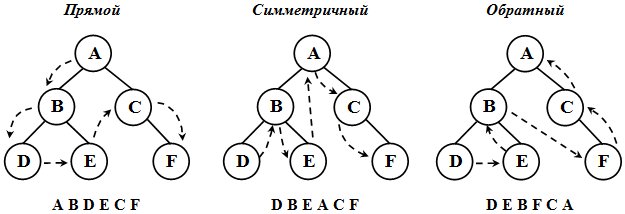
\includegraphics[width=13cm]{pic/31_02.png}

\end{figure}

\section{Приклади обчислень}
\nopagebreak[4]




\subsection*{Контрольні запитання}
\nopagebreak[4]
\begin{enumerate}
\item ?
\end{enumerate}



